\documentclass[tikz,border=5mm]{standalone}
\usepackage{amsmath}
\usepackage{tikz}
\usetikzlibrary{decorations.pathmorphing,arrows.meta}

\begin{document}

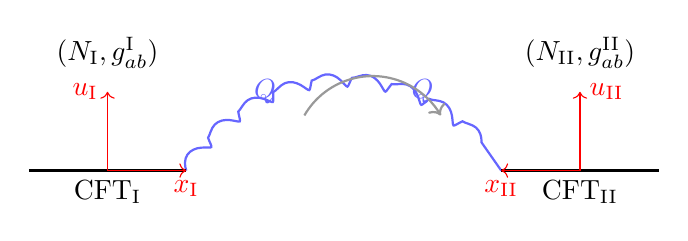
\begin{tikzpicture}
    % Define colors
    \definecolor{blueQ}{rgb}{0.4,0.4,1}
    \definecolor{redCoord}{rgb}{1,0,0}
    \definecolor{grayArrow}{rgb}{0.6,0.6,0.6}

    % Draw the interface brane Q
    \draw[blueQ, thick, decoration={coil,aspect=0.5,segment length=5mm,amplitude=1mm},decorate] 
        (-2,0) .. controls (-1,1.5) and (1,1.5) .. (2,0);
    
    % Draw the bulk regions
    \draw[thick] (-4,0) -- (-2,0) node[midway, below] {CFT$_{\text{I}}$};
    \draw[thick] (2,0) -- (4,0) node[midway, below] {CFT$_{\text{II}}$};

    % Labels for the bulks
    \node at (-3,1.5) {$(N_{\text{I}}, g_{ab}^{\text{I}})$};
    \node at (3,1.5) {$(N_{\text{II}}, g_{ab}^{\text{II}})$};

    % Coordinate systems
    \draw[redCoord,->] (-3,0) -- (-3,1) node[left] {$u_{\text{I}}$};
    \draw[redCoord,->] (-3,0) -- (-2,0) node[below] {$x_{\text{I}}$};

    \draw[redCoord,->] (3,0) -- (3,1) node[right] {$u_{\text{II}}$};
    \draw[redCoord,->] (3,0) -- (2,0) node[below] {$x_{\text{II}}$};

    % Interface labels
    \node[blueQ] at (-1,1) {$Q$};
    \node[blueQ] at (1,1) {$Q$};

    % Gray arrow
    \draw[grayArrow, thick, ->] (-0.5,0.7) arc[start angle=150,end angle=30,radius=1];

\end{tikzpicture}

\end{document}